%%%%%%%%%%%%%%%%%%%%%%%%%%%%%%%%%%%%%%%%%%%%
% En 'inclues.tex' se encuentran la importación de paquetes necesarios
%%%%%%%%%%%%%%%%%%%%%%%%%%%%%%%%%%%%%%%%%%%%
%%%%%%%%%%%%%%%%%%%%%%%%%%%%%%%%%%%%%%%%%
% University Assignment Title Page 
% LaTeX Template
% Version 1.0 (27/12/12)
%
% This template has been downloaded from:
% http://www.LaTeXTemplates.com
%
% Original author:
% WikiBooks (http://en.wikibooks.org/wiki/LaTeX/Title_Creation)
%
% License: CC BY-NC-SA 3.0 (http://creativecommons.org/licenses/by-nc-sa/3.0/)
% 
% Instructions for using this template:
% This title page is capable of being compiled as is. This is not useful for 
% including it in another document. To do this, you have two options: 
%
% 1) Copy/paste everything between \begin{document} and \end{document} 
% starting at \begin{titlepage} and paste this into another LaTeX file where you 
% want your title page.
% OR
% 2) Remove everything outside the \begin{titlepage} and \end{titlepage} and 
% move this file to the same directory as the LaTeX file you wish to add it to. 
% Then add \input{./title_page_1.tex} to your LaTeX file where you want your
% title page.
%
%%%%%%%%%%%%%%%%%%%%%%%%%%%%%%%%%%%%%%%%%
%\title{Title page with logo}
%----------------------------------------------------------------------------------------
%	PACKAGES AND OTHER DOCUMENT CONFIGURATIONS
%----------------------------------------------------------------------------------------
\documentclass[14pt]{extarticle}
%Paquetes para idioma español y codifcación UTF8
\usepackage[spanish]{babel}
\usepackage[utf8]{inputenc}
\usepackage{csquotes}

%%% BIBLATEX
\usepackage{biblatex}
%%% BIBLIOGRAPHY
\addbibresource{references.bib}

%fuente 'fourier'
\usepackage{fourier}
%paquete para URLs
\usepackage{url}
\usepackage[hidelinks]{hyperref}
%paquete para ubicar las imágenes
\usepackage{float}
%paquete para imágenes y en dónde las tiene que buscar
\usepackage{graphicx}
\graphicspath{{images/}}
%paquete para epígrafes
\usepackage{subcaption}
%paquete para definir los márgenes de la hoja
\usepackage[left=1.5cm,right=1.5cm,top=3cm,bottom=3cm]{geometry}
%paquete para poner todos y comentarios
\usepackage[colorinlistoftodos]{todonotes}
%paquete para trabajar con código
\usepackage{listings}
%paquete para trabajar con colores y definir propios
\usepackage{color}

%paquete para el checkmark y la cruz
\usepackage{pifont}
%paquete para el signo de copyright
\usepackage{textcomp}

%Cabeceras
\usepackage{fancyhdr}
\pagestyle{fancy}
\fancyhead[L]{Paradigmas de Lenguajes y Programación, 2018}
\fancyhead[C]{}
\fancyhead[R]{UNPSJB}

\fancyfoot[R]{Luciano Serruya Aloisi}
\fancyfoot[L]{Trabajo de investigación}

%Comando para poner doble comillas más fácil
\newcommand{\dq}[1]{``#1''}
\newcommand{\cmark}{\ding{51}}
\newcommand{\xmark}{\ding{55}}
\newcommand{\docker}{Docker\textregistered}
\newcommand{\doccom}{Docker-Compose\textregistered}

\definecolor{comment-green}{rgb}{0,0.5,0}
\definecolor{bg-light-gray}{HTML}{E9E9E9}
\definecolor{gopher}{HTML}{D0B698}

%% Golang definition for listings
%% http://github.io/julienc91/lstlistings-golang
%%
\RequirePackage{listings}

\lstdefinelanguage{Golang}%
  {morekeywords=[1]{package,import,func,type,struct,return,defer,panic,%
     recover,select,var,const,iota,},%
   morekeywords=[2]{string,uint,uint8,uint16,uint32,uint64,int,int8,int16,%
     int32,int64,bool,float32,float64,complex64,complex128,byte,rune,uintptr,%
     error,interface},%
   morekeywords=[3]{map,slice,make,new,nil,len,cap,copy,close,true,false,%
     delete,append,real,imag,complex,chan,},%
   morekeywords=[4]{for,break,continue,range,goto,switch,case,fallthrough,if,%
     else,default,},%
   morekeywords=[5]{Println,Printf,Error,Print,},%
   sensitive=true,%
   morecomment=[l]{//},%
   morecomment=[s]{/*}{*/},%
   morestring=[b]',%
   morestring=[b]",%
   morestring=[s]{`}{`},%
   }


\lstdefinestyle{go}{
    language=Golang,
    backgroundcolor=\color{gopher},
    basicstyle=\ttfamily,
  	keywordstyle=\bfseries\color{white},
    stringstyle=\color{blue},
    commentstyle=\color{comment-green}\itshape,
    numberstyle=\color{gray},
    identifierstyle=\color{black},
    rulecolor=\color{gray},
    showstringspaces=false,
    escapeinside={\%*}{*)},
    morekeywords={},
    otherkeywords={},
    breaklines=true,
    frame=trbl, 
    framexleftmargin=25pt,
    numbers=left,
    xleftmargin=\parindent,
    frameround=tttt,
    captionpos=b,
    % re tirado de los pelos, pero es lo que hay
    % sacado de:
    % https://tex.stackexchange.com/questions/24528/having-problems-with-listings-and-utf-8-can-it-be-fixed
    inputencoding=utf8,
    extendedchars=true,
    literate={á}{{\'a}}1 {é}{{\'e}}1 {í}{{\'i}}1 {ó}{{\'o}}1 {ú}{{\'u}}1,
}



\begin{document}

%%%%%%%%%%%%%%%%%%%%%%%%%%%%%%%%%%%%%%%%%%%%
% En 'titlepage.tex' se encuentra la página de título
%%%%%%%%%%%%%%%%%%%%%%%%%%%%%%%%%%%%%%%%%%%%
\begin{titlepage}

    \newcommand{\HRule}{\rule{\linewidth}{0.5mm}} % Defines a new command for the horizontal lines, change thickness here

    \center % Center everything on the page
     
    %----------------------------------------------------------------------------------------
    %	HEADING SECTIONS
    %----------------------------------------------------------------------------------------

    \textsc{\LARGE UNPSJB}\\[1cm] % Name of your university/college
    \textsc{\Large Licenciatura en Sistemas OPGCPI}\\[0.5cm] % Major heading such as course name
    \textsc{\large Paradigmas de Lenguajes y Programación}\\[0.5cm] % Minor heading such as course title

    %----------------------------------------------------------------------------------------
    %	TITLE SECTION
    %----------------------------------------------------------------------------------------

    \HRule \\[0.4cm]
    {\huge \bfseries Trabajo de investigación}\\[0.4cm] % Title of your document
    {\large \bfseries Go}\\[0.4cm] % Title of your document
    \HRule \\[1.5cm]
     
    %----------------------------------------------------------------------------------------
    %	AUTHOR SECTION
    %----------------------------------------------------------------------------------------


    \begin{minipage}[l]{0.5\textwidth}
        \begin{flushleft}
            \textbf{\textsf{Cátedra}}\\
            \large Lic. Romina Stickar\\ 
            \large Lic. Lautaro Pecile\\ 
            \linespread{4}
            \end{flushleft}
    \end{minipage}
    \begin{minipage}[l]{0.4\textwidth}
        \begin{flushright}
            \textbf{\textsf{Integrantes:}}\\
            \linespread{1}
            \large Luciano Serruya Aloisi\\
        \end{flushright}
    \end{minipage}\\[1.5cm]

    % If you don't want a supervisor, uncomment the two lines below and remove the section above
    %\Large \emph{Author:}\\
    %John \textsc{Smith}\\[3cm] % Your name

    %----------------------------------------------------------------------------------------
    %	DATE SECTION
    %----------------------------------------------------------------------------------------

    {\large \today}\\[1cm] % Date, change the \today to a set date if you want to be precise

    %----------------------------------------------------------------------------------------
    %	LOGO SECTION
    %----------------------------------------------------------------------------------------

    
\includegraphics[scale=1]{logoUnpsjb.png}\\[0.5cm] % Include a department/university logo - this will require the graphicx package
     
    %----------------------------------------------------------------------------------------

    % \vfill % Fill the rest of the page with whitespace

\end{titlepage}


%%%%%%%%%%%%%%%%%%%%%%%%%%%%%%%%%%%%%%%%%%%%
% INDICE
%%%%%%%%%%%%%%%%%%%%%%%%%%%%%%%%%%%%%%%%%%%%
\clearpage
\tableofcontents
\clearpage 

\lstset{style=go}

\section{Introducción}

En el año 2007, tres ingenieros de Google (\emph{Robert Griesemer}, \emph{Rob Pike}, y \emph{Ken Thompson}) comenzaron a diseñar el lenguaje de programación \emph{Go}, como proyecto secundario. Para el 2008, empezaron con el desarrollo de un compilador y un \emph{runtime} \footnote{Software diseñado para soportar la ejecución de programas escritos en algún lenguaje de programación \autocite{Wikipedia:runtime}}. El 30 de Octubre de 2009, Rob Pike dio la primer charla sobre Go en una \emph{Google Techtalk} \autocite{TheGoProgrammingLanguage}, pero recién para el 10 de Noviembre de ese mismo año el proyecto fue oficialmente anunciado. Debido a que el proyecto es \emph{open-source}, se formó una gran comunidad que aceleró el desarrollo y uso del lenguaje 

A partir de Mayo de 2010, Google utiliza Go en producción para la infraestructura de sus servidores (lo cual demuestra que la empresa apuesta en él, y que el lenguaje tiene peso como para estar en producción \autocite{TheWayToGo})

\vspace*{10mm}
\begin{lstlisting}[title=\dq{Hola mundo} en Go]
package main

import "fmt"

func main() {
    fmt.Println("Hello world!")
}
\end{lstlisting}


Sus creadores decidieron encarar el proyecto al ver que no había surgido ningún lenguaje de programación (de bajo nivel pero con amplios niveles de abstracción) que sea adeacuado para el panorama computacional de hoy en día. Por lo tanto, se considera a Go como \dq{el C del siglo 21} \autocite{BookTheGoProgrammingLanguage} 

El lenguaje se utiliza mucho para construir servidores, herramientas y sistemas para programadores, pero no deja de ser un lenguaje de propósito general.

Existen muchos lenguajes de programación que influenciaron distintas decisiones de diseño de Go, siendo alguno de ellos C (sintaxis, sentencias de flujo de control, tipos de datos básicos, \textbf{pasaje de parámetros por copia}, punteros), pero también Pascal, Modula-2 (sistema de paquetes), y CSP (manejo de concurrencia)

\begin{figure}[H]
    \centering
    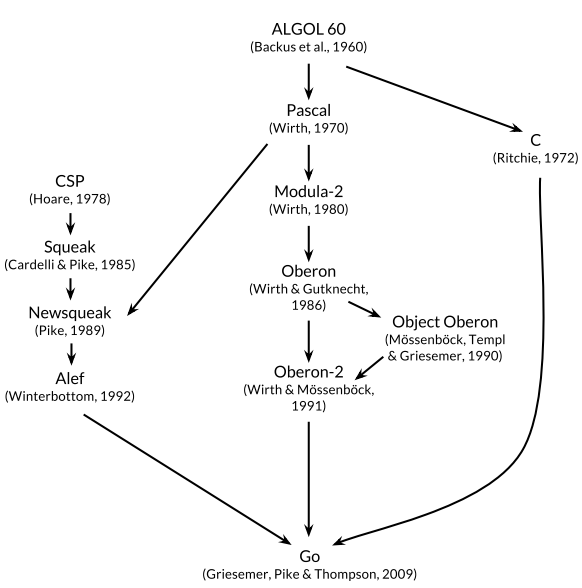
\includegraphics[width=0.8\linewidth]{ancestros.png}
    \caption{Ancestros de Go \autocite{BookTheGoProgrammingLanguage}}
    \label{fig:name}
\end{figure}


\section{Criterios de evaluación}

Go tiene una sintaxis consisa y regular, conseguida con pocas palabras reservadas. Esto aumenta la velocidad de compilación (las sentencias pueden ser evaluadas por la gramática sin una \emph{tabla de símbolos}), y reduce las líneas de código; una especificación completa del lenguaje puede hallarse en \autocite{GolangSpec}. También intenta establecer un o dos formas para realizar una determinada tarea, lo cual logra que \textbf{facilita la lectura del código}.

El lenguaje es lo suficientemente inteligente como para \emph{inferir tipos} en asignaciones con el operador \dq{:=}. Esta característica favorece a la \textbf{escritura} del código.  

\begin{lstlisting}[title=Distintas formas de declarar una variable]
s := ""
var s string
var s = ""
var s string = ""
\end{lstlisting}

El diseño y la implementación del lenguaje favorecen más que nada a la \textbf{seguridad} y al \textbf{costo de ejecución} de los programas. Para ello utiliza un \emph{recolector de basura} (\emph{Garbage Collector}), que se encarga de administrar el uso de la memoria para evitar \emph{referencias colgantes} o \emph{memory leaks} (se podría considerar también como un incremento en la facilidad de escritura)   

Go ha reemplazado lenguajes dinámicos porque balancea \emph{expresividad} con \emph{seguridad}; los programas escritos en Go típicamente corren más rápido que programas escritos en lenguajes dinámicos y sufren muchos menos errores en tiempo de ejecución por problemas de tipos inesperados \autocite{BookTheGoProgrammingLanguage}. La seguridad que provee el lenguaje se da gracias a su \textbf{sistema de tipos} y a que es \textbf{\emph{memory-safe}} (manejo de memoria seguro) \autocite{TheGoProgrammingLanguage}. 

\section{Sistema de tipos}

Go es un lenguaje \textbf{fuerte y estáticamente tipado}. Todas las expresiones tienen un tipo determinado en tiempo de compilación, y una vez declarada una variable no puede cambiar su tipo.

\vspace*{5mm}
\begin{lstlisting}[title=\centering Ejemplos de asignaciones válidas e inválidas (nótese el uso de los operadores \dq{:=} y \dq{=})]
aString := "Hello world" // Variable de tipo cadena

aString := 3 // No se puede redefinir la variable
aString := "Bye" // No se puede redefinir la variable
aString = 3 // Asignación ilegal
aString = "Bye world" // Asignación válida

\end{lstlisting}

No provee conversiones implícitas, por lo cual no es posible tener \textbf{expresiones mixtas} \footnote{expresiones que involucren más de un tipo de dato}. Tampoco tiene constructores o destructores, pero cuando se crea una variable se la inicializa con el \textbf{valor cero} o \textbf{valor inicial} de su tipo de dato.

\subsection{Tipos de datos}

Go provee distintos tipos de datos simples por defecto, ellos son:

\begin{itemize}
    \item Numéricos: su valor inicial es 0
    \begin{itemize}
        \item Enteros: con y sin signo; también brinda opciones dependientes de la plataforma
        \item Punto flotante: 32 o 64 bits.
    \end{itemize}
    \item Cadenas: se inicializan a cadena vacía ("")
    \item Booleanos: se inicializan a \texttt{false} 
\end{itemize}

Tipos de datos complejos provistos por el lenguaje son los \textbf{arreglos} (listas indexables de un tipo de dato específico con un tamaño predeterminado), las \textbf{rebanadas} o \textbf{slices} (segmento de un arreglo, su tamaño puede variar en tiempo de ejecución), y los \textbf{mapas} (listas asociativas o \emph{clave-valor}, se definen con un tipo de dato para la clave y otro para el valor). Cabe aclarar que el tamaño de un arreglo forma parte de la definición de su tipo, por lo tanto no se puede asignar a una variable cuyo tipo sea un arreglo de tamaño \texttt{X} un arreglo de tamaño distinto de \texttt{X} 

También existe la posibilidad de definir \textbf{estructuras} o \textbf{registros}, cuyos campos serán de un tipo de dato simple o complejo.

\vspace*{5mm}
\begin{lstlisting}[title=Definición de un tipo de registro \texttt{Circle} con tres campos del mismo tipo]
type Circle struct {
    x, y, r float64
}
\end{lstlisting}

Los tipos de datos complejos se inicializan con los valores iniciales que tengan los tipos de datos que los componen.

Otro tipo de dato complejo que provee Go es el tipo de dato \textbf{puntero}. Se define en base a otro tipo de dato, y su valor será el de una \textbf{dirección} de memoria que almacenará un valor del tipo de dato definido para el puntero. 

Al igual que C, se obtiene el valor apuntado por el puntero mediante el operador \texttt{*}, y para conseguir la dirección de un tipo de dato se utiliza el operador \texttt{\&} 



\section{Estructuras de control}

Go cuenta con tres estructuras de control, dos de selección y una de iteración.

La única estructura de control que implementa es el ciclo \texttt{for}, con la siguiente sintaxis:

\begin{lstlisting}[title=\centering Sintaxis del ciclo \texttt{for} (la llave debe estar en la misma línea que las sentencias de incremento)]
for <INICIALIZACIÓN>; <CONDICIÓN>; <INCREMENTO> {
    // Cero o más sentencias
} 
\end{lstlisting}

Con esta única estructura se puede simular el ciclo \texttt{while} (solamente especificando la condición, y controlándola dentro del bloque de sentencias), o un ciclo infinito (\texttt{for} sin ninguna indicación) 

Si se desea iterar sobre una estructura indexable (arreglo o mapa), la claúsula \texttt{range} devuelve una clave y su respectivo valor   

\vspace*{5mm}
\begin{lstlisting}[title=Iterando sobre un arreglo con \texttt{range}]
for i, value := range arr {
    fmt.Printf("POSICION %d : VALOR %v\n", i, value)
} 
\end{lstlisting}

La estructura de decisión más simple con la que cuenta el lenguaje es el \texttt{if}. Al igual que el \texttt{for}, la condición no necesariamente se escribe entre paréntesis, y las llaves que indican el bloque de instrucciones son necesarias y van en la misma línea que la condición. Se puede indicar también, con la palabra reservada \texttt{else}, el bloque de sentencias a ejecutar si no se cumple la condición especificada por el \texttt{if}.  

\vspace*{5mm}
\begin{lstlisting}[title=Ejemplo de varias estructuras de control]
for i := 0; i < 10; i++ {
    if i % 2 == 0 {
        fmt.Printf("El valor %d es par\n", i)
    } else {
        fmt.Printf("El valor %d es impar\n", i)
    }
}
\end{lstlisting}

Otra estructura de decisión es el \texttt{switch}; consiste en indicar una \emph{sentencia simple} \footnote{sentencia que devuelva un valor}, dentro de las llaves los distintos casos posibles con la palabra \texttt{case} y seguido de dos puntos (:) el bloque de sentencias que se desea ejecutar si se cumple esa condición. 

El comportamiento por defecto del \texttt{switch} es distinto al \texttt{switch} de C, en tanto que si se cumple una condición, no seguirá automáticamente ejecutando el bloque de sentencias de la condición que esté por debajo de la que se cumplió (si se desea tal comportamiento, se lo puede especificar con la palabra \texttt{fallthrough} \autocite{TheWayToGo}).

Por último, se puede especificar un bloque de sentencias a ejecutar si ninguna de las condiciones anteriores se cumplieron; tal bloque se indica con la palabra reservada \texttt{default} 

\begin{lstlisting}[title=Estructura de decisión múltiple \texttt{switch}]
switch var1 {
    case val1:
        ...
    case val2:
        ...
    default:
        ...
}
\end{lstlisting}


\section{Paradigmas}

Principalmente, Go es un lenguaje de programación \textbf{procedural}. Utiliza estructuras de control, asignación de variables, constantes, y funciones que manipulan datos.

Las funciones pueden recibir cero o más parámetros de cualquier tipo, y pueden devolver o más resultados (la expresión \texttt{range} devuelve dos valores, el índice de una estructura iterable y su correspondiente valor). La cantidad de parámetros que recibe una función puede ser variable, especificándolo con \texttt{...} antes del tipo del parámetro.

\vspace*{5mm}
\begin{lstlisting}[title=Función con cantidad variable de argumentos]
func sumatoria(args ...int) int{
    total := 0
    for _, value := range args {
        total += value
    }
    return total
}
\end{lstlisting}

La firma de una función siempre empieza con la palabra reservada \texttt{func}, le sigue el nombre de la función, luego entre paréntesis los argumentos que recibe, indicando primero su nombre y después su tipo (si es que recibe parámetros, si no recibe se dejan los paréntesis vacíos), y por último el resultado que devuelve (si son varios, se especifica entre paréntesis el tipo de dato de cada valor devuelto). 

Go considera las funciones como \emph{ciudadanos de primera clase} \autocite{Wikipedia:first-class-citizen}, por lo tanto pueden ser recibidas como parámetros (una función puede recibir una función), o devueltas como resultado (una función que devuelve una función\footnote{El patrón de diseño \emph{Decorador} podría ser implementado gracias a esta característica}) 

El lenguaje también permite definir \emph{funciones anónimas}; su definición se trata como una expresión. Se pueden almacenar en variables, y no llevan nombre. 

Antes del nombre de una función, se puede especificar \emph{el tipo de dato receptor}, lo cual convertiría a la función en un \emph{método}. De esta forma, se pueden agregar comportamientos a los tipos de datos definidos por el usuario (aunque puede ser casi cualquier tipo de dato \autocite{TheWayToGo:Methods})

\Large The Way to Go página 240 (265 del PDF)

\section{Manejo de eventos inusuales}


\section{Concurrencia}
\subsection{\texttt{goroutines}}
\subsection{Canales}













%%%%%%%%%%%%%%%%%%%%%%%%%%%%%%%%%%%%%%%%%%%%
% FIN DOCUMENTO, AHORA REFERENCIAS
%%%%%%%%%%%%%%%%%%%%%%%%%%%%%%%%%%%%%%%%%%%%
\clearpage
\printbibliography

\end{document}

